\chapter{Componente tecnologica}
\section{Introduzione}
La realizzazione del progetto prevede, dopo la definizione di una precisa architettura, l'utilizzo di diverse componenti tecnologiche, come ad esempio l'utilizzo di un framework, per soddisfare i vari requisiti utente.
\section{Strumenti utilizzati per l'organizzazione del lavoro}
\subsection{ClickUp}
Ai fini di organizzare per il meglio il lavoro da svolgere, l'utilizzo della piattaforma ClickUp ha permesso al team di sviluppo la suddivisione dei compiti da svolgere mediante la definizione di macro-task, organizzati in dashboard visibili dal settore amministrativo e tecnico. Un macro-task rappresenta l'implementazione di un caso d'uso utente e corrisponde ad un rilascio in produzione. Inoltre prevede un'univocità all'interno della dashboard ed è visibile e modificabile dal reparto di amministrazione per supervisionare l'andamento del progetto. A sua volta un macro-task è suddiviso in task, i quali sono organizzati nei diversi pannelli (admin, negozio, utente, comune) riprendendo il codice univoco a cui è associato il macro-task. Ogni task è inserito nella dashboard gestita dal team di sviluppo e corrisponde all'implementazione di una micro-funzionalità. Deve soddisfare precisi requisiti, di seguito elencati.
\begin{itemize}
    \item \textbf{Durata Limitata}: un task deve prevedere un tempo di implementazione da una alle quattro ore complessive
    \item \textbf{Atomicità}: un task deve prevedere l'implementazione/correzione di funzionalità singole
    \item \textbf{Univocità}: un task non deve essere mai ripetuto, per implementare bugfixes è necessario creare un nuovo macro-task e di seguito organizzarne la suddivisione
    \item \textbf{Reperibilità}: un task deve essere facilmente trovato ricercando parole chiave definite nel titolo, il quale segue lo standard <<\textit{COD \# - Titolo breve}>>
\end{itemize}
Ogni task nel flusso di lavoro può assumere diversi status:
\begin{itemize}
    \item \textbf{Open}: il task è appena stato creato e non è ancora stato implementato
    \item \textbf{In Progress}: il task è in corso di implementazione da parte del team di sviluppo
    \item \textbf{Review}: il task è in corso di revisione da parte dei preposti al testing
    \item \textbf{Closed}: il task è concluso e testato
\end{itemize} 
Un macro-task può passare nello status "closed" solo quando tutti i task a lui relativi sono in closed. A questo punto è possibile procedere con il rilascio della piattaforma in produzione.
\begin{figure}[!htb]
    \centering
    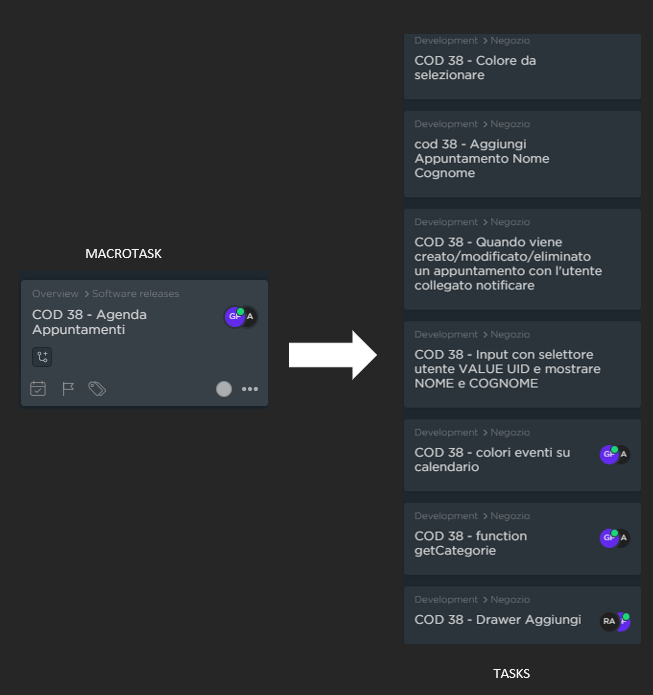
\includegraphics[width=0.7\textwidth]{divis.png}
    \caption{Esempio di organizzazione macrotask - tasks di una funzionalità di Garzone}
\end{figure}
\subsection{Bitbucket}
Per consentire la condivisione ddel codice sorgente tra il team di sviluppo è stato previsto l'utilizzo della piattaforma Bitbucket, un servizio di hosting per progetti implementati tramite utilizzo del protocollo di version control Git. Per l'implemntazione del progetto sono state create quattro apposite repository:
\begin{itemize}
    \item \textbf{garzone-serverless}: la quale comprende tutto il codice sorgente relativo alla componente backend
    \item \textbf{garzone-webapp-admin}: relativo al pannello admin
    \item \textbf{garzone-webapp-negozio}: relativo al pannello negozio
    \item \textbf{garzone-webapp-comune}: relativo al pannello comune
    \item \textbf{garzone-webapp-utente}: relativo al pannello utente
\end{itemize}   
Le operazioni di version control sono state effettuate tramite l'utilizzo di Github Desktop, un'applicazione che utilizza il protocollo Git mediante un'interfaccia grafica. Ad ogni task del progetto implementato è correlato un commit creando quindi un riferimento al flusso di lavoro definito in partenza. 
\subsection{Separazione ambienti di lavoro}
La separazione degli ambienti di lavoro è necessaria per permettere al team di sviluppo di lavorare alle implementazioni di test parallelamente a quelle in produzione. In questo modo si consente un corretto utilizzo della piattaforma da parte dell'utenza su una versione testata e la possibilità da parte degli sviluppatori di procedere con il live deploy solo dopo aver testato il deploy di test. Al progetto vero e proprio firebase-hosted ne è stato quindi affiancato un altro parallelo, il quale presenta lo stesso identificativo \textit{(piattaforma-garzone)} con l'aggiunta del suffisso \textit{"-test"}. I due progetti presentano la medesima suddivisione di sottodomini e si interfacciano a backend differenti, i quali a loro volta si interfacciano a due istanze di basi di dati differenti.
Per l'avvio e la sua messa in produzione, il progetto prevede l'utilizzo di script appositi per ogni pannello, ognuno dei quali ha una funzione specifica di avvio o di deploy. Di seguito vengono proposti gli script relativi alla parte di backend e relativi alla componente frontend del pannello utente, seguiti da una panoramica generale dei servizi a cui si interfacciano le varie piattaforme.
\begin{figure}[!htb]
    \centering
    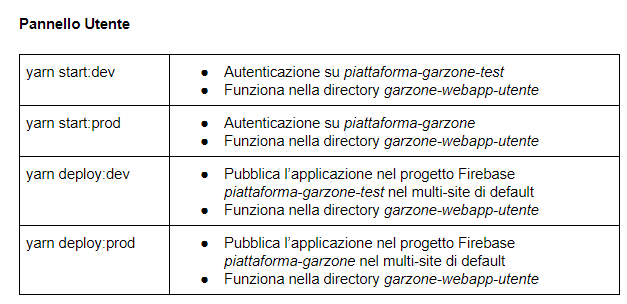
\includegraphics[width=0.8\textwidth]{ut.png}
    \caption{Documentazione degli script di avvio/deploy del pannello utente}
\end{figure}
\begin{figure}[!htb]
    \centering
    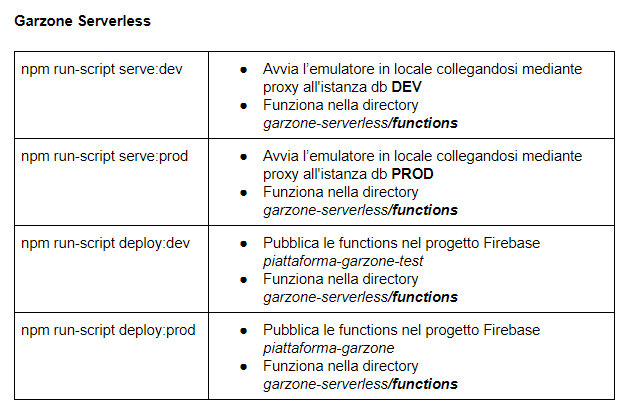
\includegraphics[width=0.8\textwidth]{serv.png}
    \caption{Documentazione degli script di avvio/deploy della componente backend (firebase functions)}
\end{figure}

\begin{figure}[!htb]
    \centering
    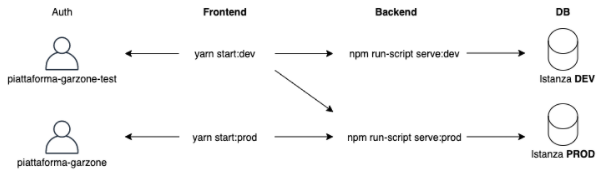
\includegraphics[width=0.8\textwidth]{env.png}
    \caption{Sommario script di avvio dei progetti di test e live e relative interfacce}
\end{figure}
\section{Javascript e NodeJS}
Il progetto è interamente realizzato tramite l'utilizzo del linguaggio Javascript. Fu introdotto nel 1995 come strumento per inserire programmi nelle pagine web del browser Netscape Navigator. Successivamente è stato via via adottato da tutti gli altri browser grafici, rendendo realizzabili moderne applicazioni Web con le quali si può interagire direttamente, senza dover necessariamente ricaricare la pagina. Vie anche utilizzato in siti più tradizionali per offrire varie forme di interattività.\cite{JS}. Node.js è stato creato tramite l'utilizzo di javascript. In particolare si tratta di un ambiente asincrono ed event driven per la costruzione di applicazioni distribuite basate su Javascript. Node.js non è un framework, lavora infatti a livelli più bassi, è sostanzialmente un 
interprete con alcune librerie di base non native del linguaggio Javascript, ad esempio per l’I/O su file, per l’implementazione di 
server per vari protocolli standard. Sfrutta il loop di gestione degli eventi di Javascript, in particolare sulla possibilità 
di definire funzioni callback per implementare uno schema di I/O non 
bloccante.
\subsection{Features introdotte in ES2021 utilizzate}
\subsection{npm}
\newpage
\section{Componente Frontend}
\subsection{Linee guida grafiche per l'interfaccia utente}
\subsection{ReactJS e antd}
\subsection{Less}
\newpage
\section{Componente Backend}
\subsection{Google Cloud}
\subsubsection{Cloud SQL}
\subsubsection{Firebase}
\subsubsection{Firebase Functions}
\subsubsection{Realtime Database}
\subsection{AWS}
\subsubsection{Simple Email Service}
\subsection{Stripe}
\subsubsection{Stripe Connect}